
\chapter{Empirical solar-wind model for the inner heliosphere}
\label{chap:empirical_solar_wind_model_for_the_inner_heliosphere}

%COFI -- chapter outline and flow integration
This chapter is constructed as follows, the PSP mission, scientific goals, and spacecraft are described, I introduce the analyses done in the publication \citet{Venzmer2017}, which belongs to this chapter, an improvement to the magnetic field solar distance dependency is derived, which deprecates that from the paper, other things, and further an outlook is given.\\

paper introduction and context of motivation in thesis and context of results in thesis\\

% from paper:
We obtained lognormal representations of the frequency distributions’ shapes of the four key solar wind parameters magnetic field strength, proton velocity, density and temperature. We derived analytical relations for the parameters’ solar activity dependencies and for their solar distance scaling. An empirical solar wind model was build from the combination of the obtained frequency distributions, SSN dependence relations and solar distance dependence functions, representing the solar wind’s solar activity and distance behavior. This empirical model was fed with SSN predictions and extrapolated to the orbit of PSP. We estimated solar wind median values during PSP’s first perihelion and modeled the values for PSP’s closest perihelia.\\
- further investigations should be done into structure extrapolations\\
- outward extension of model seems feasable (e.g., to Mars)\\
In order to derive the solar wind environment for the PSP orbit, finally the general solar wind model derived in the previous sections will be extrapolated to the PSP orbit, taking into account predictions of the SSN.\\
varying shape with distance is indicator for internal physical processes (mixing/turbulence...)\\



%%% contributions and copyright
The major part of this chapter is published in \citet{Venzmer2017} ((replace arXiv cite with aanda's)). The paper, published in Astronomy and Astrophysics (A\&A), is included following this chapter and \textbf{not yet} reproduced with permission \textcopyright~ESO.

The analyses described in the paper were entirely done by me, as well as the tables, figures and equations. My coauthor Volker~Bothmer contributed to the text and the anonymous referee helped clarifying a few aspects. The text was further improved by the A\&A language editor Joshua~Neve.\\
% my own contributions to the paper (percentages):\\
% data analyses 100\\
% tables 100\\
% figures 100\\
% formulas 100\\
% section structure 80\\
% text 55\\
% - abstract 70\\
% - introduction 30\\
% - frequency distributions 65\\
% - solar activity dependence 70\\
% - solar distance dependency 60\\
% - empirical solar wind model 75\\
% - model extrapolation 35\\
% - discussion and summary 20\\


\section{Parker Solar Probe mission}

include photo/picture\\
Sun angular diameter comparison, see presi S³\\


\section{Solar distance dependency---theory}
B-field radial profile: $B \propto r^{-1.5?}$\\
	Magnetic field magnitude model (Kivelson 1995):\\
	Br(r) = B0 / r²\\
	Bphi(r) = -B0 omega / (Vr * r) (shear effect from solar rotation omega)\\
	Btheta(r) = 0\\
	B(r) = (Br² + Bphi² + Btheta²)**1/2\\
	B(r) = sqrt((B0 / r²)² + (-B0 omega / (Vr * r))²)	--> expected r dependency: B propto a*r**-2 + b*r**-1\\
	Parker references\\
velocity radial profile: $V \propto r^{0?}$\\
	model based on LeBlanc1998 electron density with flux conservation: Zic2015(Temmer)\\
density radial profile: $N \propto r^{-2}$\\
	simple view: for a spherical constant velocity mass outflow a one over distance squared law is expected, because of the mass flux conservation per solid angle for different distances. measurements up to the outer heliosphere confirm the $1/r^2$ dependency (1--38~au by Voyager~2, \citep{Belcher1993} newer paper?)\\

	in an ideal neutral plasma the electron and proton number density have the same values (neutral plasma) (reference?)\\
	ca. 10~\% more electrons than protons (due to alphas) cite?\\	%http://omniweb.gsfc.nasa.gov/ftpbrowser/bow_derivation.html\\
temperature radial profile: $T \propto r^{-1?}$\\
	at larger distances heating outbalances the adiabatic temperature part (adiabatic cooling vs. pickup proton and stream--interaction heating; 1--68~au by Voyager~2; \citet{Richardson2003}\\
solar wind ram pressure $p_\text{ram} = \rho V^2$\\


\section{Outlook}

- implement flux conservation ($v$ and $n$ relation) into radial distance dependencies\\
- implement velocity dependent magnetic field strength into radial distance dependency\\


\subsection{flux conservation}
conserved quantities:\\
- momentum conservation... VBbookp112\\
- flux conservation...\\

%%%%%%%%%%%--  flux  --%%%%%%%%%%%%%%%
%As Schwenn1983 stated ``From Helios in situ measurements we know that at least beyond 0.29~au there is almost no nonradial flow, on the average. In fact, the particle flux was found to be that quantity which varies the least with increasing R.''\\

%Schwenn1990:
%increase in sw velocity with distance; speed increase mainly in slow solar wind
%density deviates from a purely r^-2 fall-off (10% faster); n(r)=6.1*r^-2.1 cm^-3; different behavior in slow and fast wind
%proton flux density constant between 0.3-1.0~au -> no meridional flow into/out of the ecliptic; different for slow and fast sw

With consideration of continuity the mass flux per solid angle has to be constant: $\dot{m} = \text{const}$\\
conserved quantities:\\
- mass flux: $\dot{m} = \rho v A$ (with mass density $\rho$, velocity $v$ and [cross-sectional area $A$] or solid angle?...)\\
- particle fluxes (proton flux, electron flux, etc.)\\
	- proton flux: $j_\text{p} = n_\text{p} v_\text{p} A$ (with proton density $n_\text{p}$ and proton velocity $v_\text{p}$)\\

(with proton mass density $\rho = n_\text{p} m_\text{p}$ (with proton number density $n_\text{p}$ and proton mass $m_\text{p}$).)\\

the individual radial dependencies for a spherical radial outflow are:\\
$A(r) \propto r^2$ --> $A/r^2 = \text{const}$\\
and assuming an exponential dependency,\\
$n_{\text{p}}(r) = n_0 r^{c_n}$,\\
$v(r) = v_0 r^{c_v}$\\
\begin{align}
	j_\text{p} &= \text{const}\\
	n_\text{p} v_\text{p} A &= \text{const}\\
	n_0 r^{c_n} v_0 r^{c_v} r^2 &= \text{const}\\
	r^{c_n} r^{c_v} r^2 &= \text{const}\\
	\Rightarrow c_n + c_v + 2 &= 0\\
	c_n + c_v &= -2
\end{align}
an increasing velocity should result in a steeper density...\\

validity of mass flux continuity: within the heliosphere mass to energy conversion and vice versa is negligible, but there can be flux from and to higher latitudes as the Helios data is localized to a small latitude range in the ecliptic plane.\\
estimate the error from that... (if error is too big => drop continuity condition)\\
larger errors should be located near CMEs and CIRs (nonradial flows from interactions)\\
there is a proton flux difference between slow and fast solar wind streams (see book Schwenn1990 p.~146)

estimate the possible size of error:\\
mean:\\
$c_n = -2.010$\\
$c_v = 0.049$\\
$c_n + c_v = -1.961$\\
difference to -2 is 0.039\\
% [median:\\
% $c_n = -2.093$\\
% $c_v = 0.058$\\
% $c_n + c_v = -2.035$\\
% difference to -2 is -0.035\\
% ]constant mass flux only for mean...\\



\subsection{Magnetic field strength solar distance dependency improvement}

in the paperMVVB it is seen that the magnetic field strength mean and median cross each other at 0.339 au and the mean is lower than the median at smaller distances, in agreement with the Parker spiral geometry of the interplanetary magnetic field (IMF)?.\\

The coronal magnetic field near the Sun rigidly rotates, holding on to the coronal plasma. At the solar wind source surface, where the thermal plasma pressure overcomes the magnetic pressure, the magnetic field gets radially transported outwards maintaining only its radial component $B_r$. From there on, the solar rotation begins to shear the magnetic field, building up a longitudinal component $B_\phi$ as well.\\

Solar wind magnetic field model of \citet{Parker1958} with its components in spherical coordinates ($\theta$ is the colatitude):
\begin{align}
	\vect{B}_r(r) &= B_0 \left(\frac{r_0}{r}\right)^2 \cdot \vect{e}_r\\
	\vect{B}_\phi(r) &= -B_0 \left(\frac{r_0}{r}\right)^2 \cdot \frac{\omega\,r\,\sin\theta}{v_\text{sw}} \cdot \vect{e}_\phi\\
	\vect{B}_\theta(r) &= 0 \cdot \vect{e}_\theta\\
	B(r) &= \sqrt{\vect{B}_r^2 + \vect{B}_\phi^2 + \vect{B}_\theta^2}\\
	B(r) &= \sqrt{\left(B_0 \left(\frac{r_0}{r}\right)^2\right)^2 + \left(-B_0 \left(\frac{r_0}{r}\right)^2 \cdot \frac{\omega\,r\,\sin\theta}{v_\text{sw}}\right)^2}\\
	B(r) &= B_0 \left(\frac{r_0}{r}\right)^2 \cdot \sqrt{1 + \left(\frac{\omega\,r\,\sin\theta}{v_\text{sw}}\right)^2}
\end{align}
with the norming field strength $B_0$ at the norming distance $r_0$. The solar angular rotation rate $\omega$ and the solar wind velocity $v_\text{sw}$.\\

In this model with increasing solar distance, its radial component scales with $r^{-2}$ as it is expected for a spherical source.\\

Thus, in the ecliptic ($\theta = 90\degree$), the field strength scales like
\begin{align}
	B(r) &= B_0\,r^{-2} \cdot \sqrt{1 + \left(\frac{\omega\,r}{v_\text{sw}}\right)^2}\\
	B(r) &= B_0 \cdot \sqrt{r^{-4} + \left(\frac{\omega}{v_\text{sw}}\right)^2 r^{-2}}\\
	B(r) &= B_0 \cdot \sqrt{r^{-4} + b\,r^{-2}}\\
	B(r) &= B_0 \cdot \sqrt{r^{-4} + r^{-2}}	\text{\,, for } b = 1\\
	B(1\,\text{au}) &= B_0 \cdot \sqrt{2}
\end{align}
with the distance in [au] and $B_0$ the radial field component at 1 au.\\

at 1 au the observed field angle in the ecliptic $\phi$ is about \SI{45}{\degree} ($B_r = B_\phi$, thus $B(1 au) = B_0 \cdot \sqrt{2}$). see theta and phi angles from the OMNI data in \autoref{fig:histogram_B_angles} and calculate omega from equation with typical values...\\
\begin{figure}[htb]
	\centering
	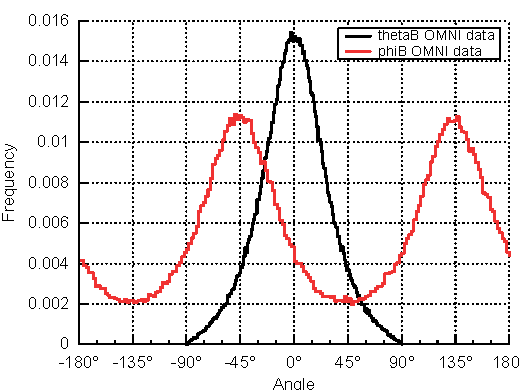
\includegraphics[width=0.5\textwidth]{images/gnuplots/histogram_B_angles.pdf}
	\caption{Magnetic field angles $\theta$ and $\phi$ in GSE coordinates.}
	\label{fig:histogram_B_angles}
\end{figure}
Therefore $\left(\frac{\omega}{v_\text{sw}}\right) = b = 1$\\
fit function: $f(r) = a \cdot \sqrt{\left(r^{e_1}\right)^2 + \left(r^{e_2}\right)^2}$\\
expected $r$-dependency: $a \approx B(1 au) / \sqrt{2}$, $e_1 \approx -2$, and $e_2 \approx -1$\\
fit function in \autoref{fig:radial_fit_B_test2} and resulting fit parameters in \autoref{tab:bfield_fit_parameters}\\
\begin{figure}[htb]
	\centering
	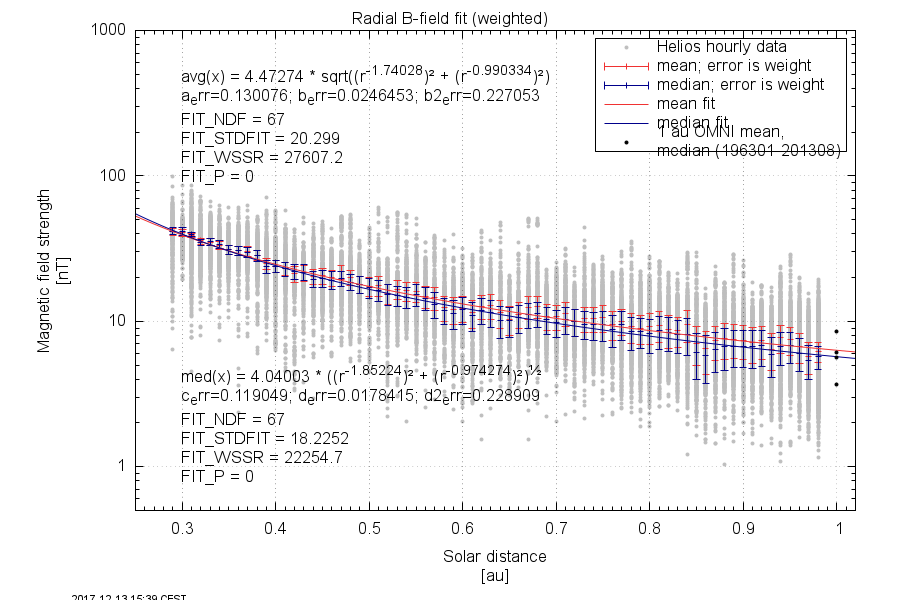
\includegraphics[width=0.5\textwidth]{images/gnuplots/radial_fit_B_test2.png}
	\caption{Helios hourly data plot of the magnetic field strength with respect to solar distance. The mean and median per \SI{0.01}{\au} data bin and their fit curves are plotted as well. The Helios data has a native distance resolution of \SI{0.01}{\au}, thus, to make the distribution visible in these plots, we added a random distance value of up to \SI{+-0.005}{\au}.}
	\label{fig:radial_fit_B_test2}
\end{figure}
\begin{table*}
	\caption{Fit parameters for the median and mean magnetic field strength solar distance relations and their crossing distance.}
	\label{tab:bfield_fit_parameters}
	\centering
	\sisetup{table-figures-integer=1, table-figures-decimal=4, table-figures-exponent=0}
	\begin{tabular}{l l c c c c}
		\hline\hline
		\multirow{2}{*}{Fit}	&	&Factor	&\multicolumn{2}{c}{Exponents}	&Crossing distance\\
		\cline{3-4}
			&	&$a$	&$e_1$	&$e_2$	&[au]\\
		\hline
		\multirow{2}{*}{Curve}	&Median	&4.04(13)	&-1.852(25)	&-0.97(23)	&\multirow{2}{*}{0.33625(??)}\\
			&Mean	&4.47(12)	&-1.740(18)	&-0.99(23)	&\\
		\multirow{2}{*}{Distribution}	&Median	&3.833(27)	&\multirow{2}{*}{-1.858(42)}	&\multirow{2}{*}{-1.32(12)}	&\multirow{2}{*}{--}\\
			&Mean	&4.081(29)	&	&	&\\
		\hline
	\end{tabular}
\end{table*}
%%% radial fit %%%
%4.47274*sqrt((r**-1.74028)**2 + (r**-0.990334)**2) = 4.04003*sqrt((r**-1.85224)**2 + (r**-0.974274)**2)\\
%r approx 0.336257719\\
%fit values
%4.04003	-1.85224	-0.974274
%4.47274	-1.74028	-0.990334
%errors
%0.130076	0.0246453	0.227053
%0.119049	0.0178415	0.228909
%table format
%4.04(13)	-1.852(25)	-0.97(23)
%4.47(12)	-1.740(18)	-0.99(23)
%avg WSSR = 27607.2	-6%
%med WSSR = 22254.7	-9%
%old avg WSSR = 29339.9	for simple power law function a*r^b
%old med WSSR = 24586.6
%
%%% fixed fit %%%
% 4.08078	-1.85771	-1.32237
% 3.83306	-1.85771	-1.32237
% errors:
% 0.0291872	0.042217	0.115887
% 0.0265236	0.042217	0.115887
% for table formatted:
% 4.081(29)	-1.858(42)	-1.32(12)
% 3.833(27)	-1.858(42)	-1.32(12)
% WSSR = 1.44202
% 1267.19055342511	this fit; is 33 % higher
% 950.841158464094	paper fit

Here, the WSSR is \SI{6}{\%}/\SI{9}{\%} lower compared to the simple power law function a*r**b in \citet{Venzmer2017}.\\

we make a distribution fit. see fit distribution in \autoref{fig:fit_B_freq_r_fixed_width} and resulting fit parameters in table X.\\
\begin{figure}[htb]
	\centering
	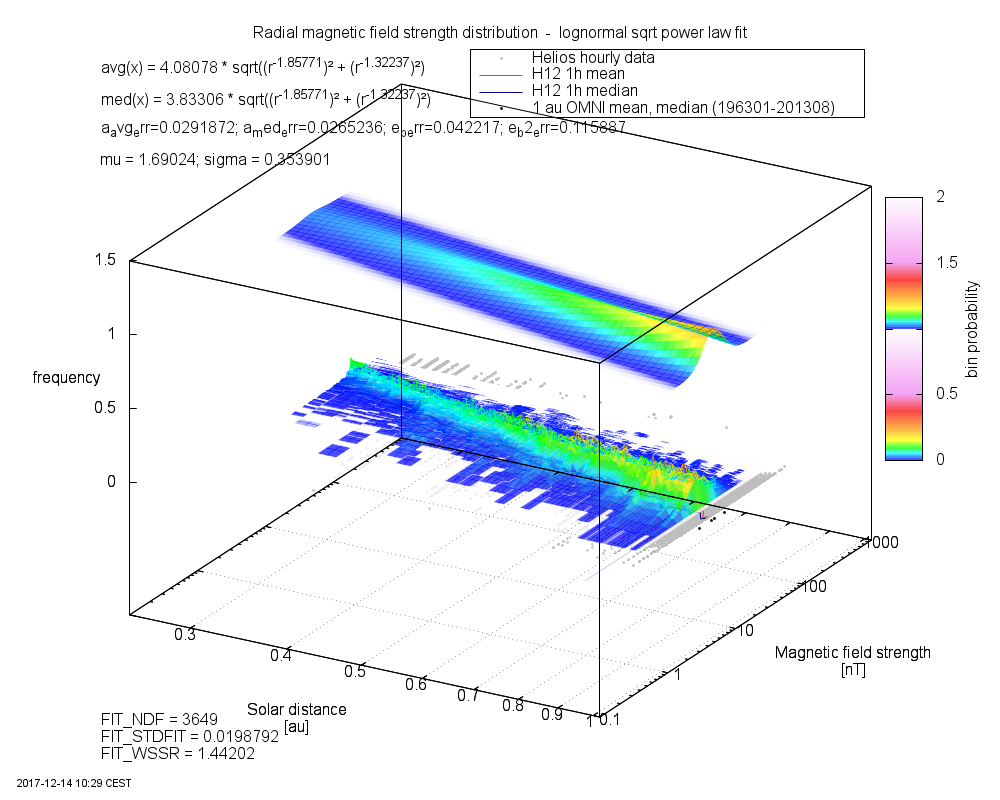
\includegraphics[width=0.5\textwidth]{images/gnuplots/fit_B_freq_r_fixed_width.png}
	\caption{Frequency distribution of the solar wind magnetic field strength with respect to solar distance. Plotted are the binned Helios data and the square-root power-law lognormal fit model with its median value (white line). replace figure...}
	\label{fig:fit_B_freq_r_fixed_width}
\end{figure}

At \SI{0.046}{\au} the median value is \SI{1267}{\nano\tesla} -- this is \SI{33}{\%} higher than the value in the paper.\\

scaling SSN-relation with the fit result: $B(ssn,r) = \frac{B(ssn)}{\sqrt{2}} \cdot \sqrt{\left(r^{e_1}\right)^2 + \left(r^{e_2}\right)^2}$\\


This result combined with the values obtained from the solar activity analysis in the paper is
\begin{align}
	B_\text{med}(ssn,r) &= \left(\SI{0.0131}{\nT} \cdot ssn + \SI{4.29}{\nT}\right) \cdot \sqrt{\left(r^{-1.86}\right)^2 + \left(r^{-1.3}\right)^2}	\,,\\
	B_\text{avg}(ssn,r) &= 1.0879 \cdot B_\text{med}(ssn,r)\,.
\end{align}

extrapolation to the PSP orbital range, see \autoref{fig:sw_extrapolation_ssn_f}\\
\begin{figure}[htb]
	\centering
	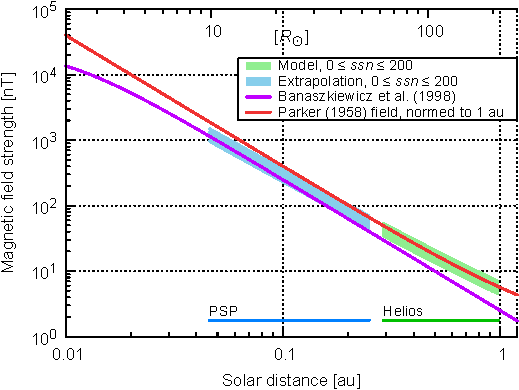
\includegraphics[width=0.5\textwidth]{images/gnuplots/sw_extrapolation_ssn_f.pdf}
	\caption{Radial extrapolation of the solar-wind magnetic field strength to the PSP orbit region. The median value from the model, obtained from Helios and OMNI measurements, is extrapolated to the PSP region for SSN values between solar minimum and maximum, that is, $0 \le ssn \le 200$. The lower edges of the shaded areas correspond to solar minimum, the upper edges to solar maximum. Also plotted are the radial dependencies of the analytic DQCS magnetic field model for solar minimum (violet) from \citet{Banaszkiewicz1998} and the Parker field model (red).}
	\label{fig:sw_extrapolation_ssn_f}
\end{figure}

forecast to PSP orbit and mission time, see autoref{fig:}\\
extrapolation to the PSP orbital range, see \autoref{fig:PSP_perihelia_prediction_f}\\
\begin{figure}[htb]
	\centering
	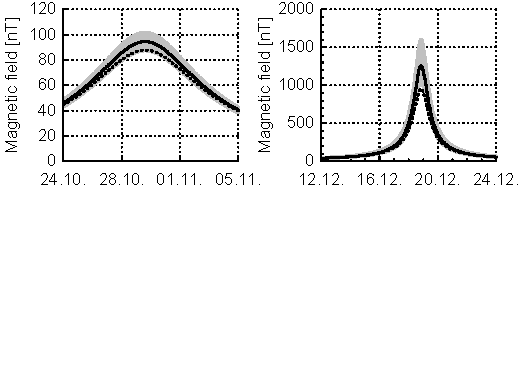
\includegraphics[width=0.5\textwidth]{images/gnuplots/PSP_perihelia_prediction_f.pdf}
	\caption{Estimated solar-wind parameter medians (solid) and their error bands (gray area) during 12~days in 2018 and 2024 with PSP's first perihelion at about \SI{0.16}{\au} and PSP's 22nd (the first closest) perihelion at \SI{0.046}{\au}. The prediction from \citet{Venzmer2017} is indicated as well (dotted).}
	\label{fig:PSP_perihelia_prediction_f}
\end{figure}
% first perihelion value:
% 94 nT	this fit; is 8 % higher
% 87 nT	old fit
% first closest perihelion value:
% 1241 nT	this fit; is 32 % higher
% 943 nT	old fit

The estimated magnetic field strength median value of \SI{94}{\nano\tesla} for the first perihelion is \SI{8}{\%} higher than that in the paper. However, the median value of \SI{1241}{\nano\tesla} for the first closest perihelion is \SI{32}{\%} higher.\\


The estimated frequency distributions of the solar-wind magnetic field strength at PSP's 1st and 22nd (first closest) perihelion are plotted in \autoref{fig:PSP_sw_distributions_b}.\\
\begin{figure}[htb]
	\centering
	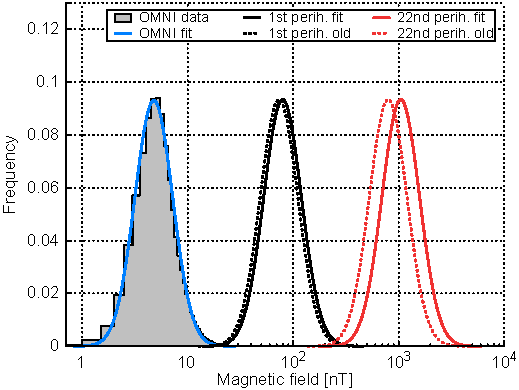
\includegraphics[width=0.5\textwidth]{images/gnuplots/PSP_sw_distributions_b.pdf}
	\caption{Frequency distributions of the solar-wind magnetic field strength (OMNI data) and those estimated with the solar-wind model for PSP's 1st and 22nd (first closest) perihelion. In these Figures the frequencies of both extrapolated curves are scaled for visibility to the same height as the \SI{1}{\au} distribution. The predictions from \citet{Venzmer2017} are indicated as well (dotted).}
	\label{fig:PSP_sw_distributions_b}
\end{figure}

\begin{figure}[htb]
	\centering
	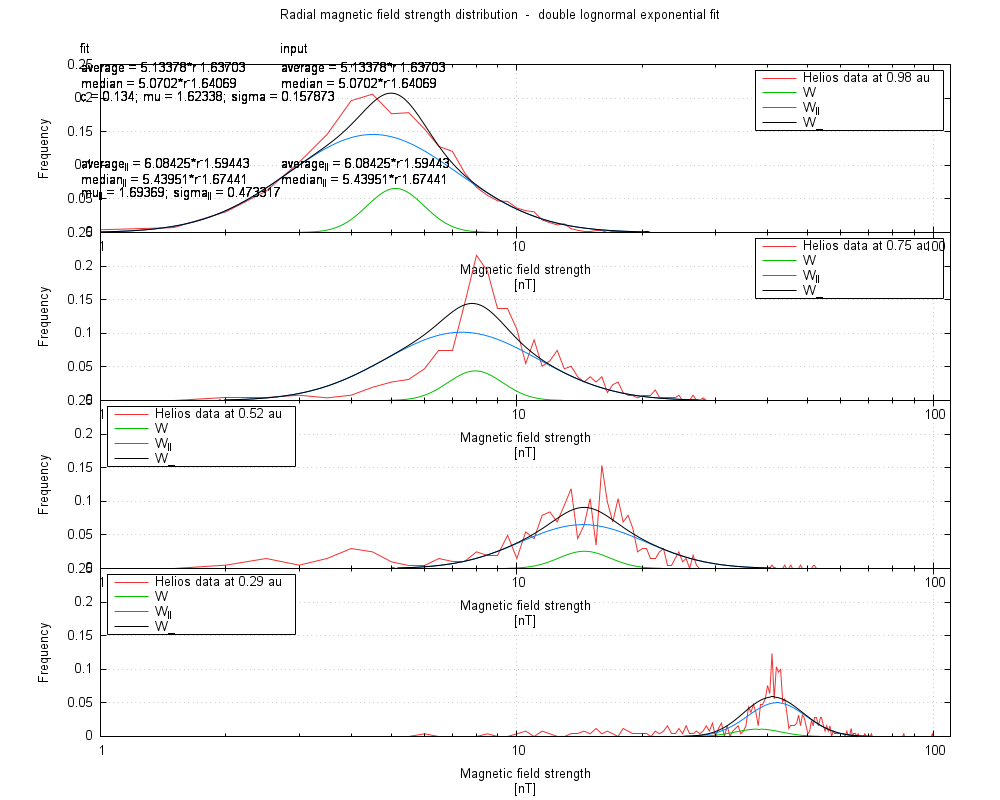
\includegraphics[width=0.4\textwidth]{images/gnuplots/double_fit_B_freq_r_plot_thesis.png}
	\caption{Plot of the magnetic field strength's frequency distribution at different solar distances (0.29, 0.52, 0.75 and 0.98~au). The Helios data, the composed fit model and both its components are plotted. 0.23~au steps, lw 2, stepfunction}
	\label{fig:double_fit_B_freq_r_plot_thesis}
\end{figure}

=> what kind of distribution has the B-field near the Sun?\\

%conclusion
The result of this analysis is that the newly derived dependency relation can be used to replace and deprecate that found in the paper.\\



\section{Literature}
Schwenn1983 intro -> sw-averaging comment (beer and wine)\\
see Hellinger2013 p.1353\\
see astro70/CGAUSS/dropbox\_presis/... (presi 1.07 Inside Helios-Origins and Evolution-Salem.ppt -> Helios reloaded; radial functions for all parameters)\\
see Balogh1999 from p. 162 (Helios CIR results)\\
see Marsch1999... (model constraints)\\
model boundary condition: continuity of mass flux\\
On solar wind acceleration and SPP proposition: McComas2007\\
Parker1963 book, p.~75 -> isothermal expansion figure\\	%https://babel.hathitrust.org/cgi/pt?id=uc1.b4264142;view=1up;seq=12

Motivational question: What is the evolution of the solar wind parameters/structures before arriving at Earth?\\
what is meant by the term evolution?\\


\section{Seasonal solar wind variations}
seasonal variation by month\\
quantify variation amplitudes\\

see \autoref{fig:OMNI_monthly_freq_V_gps}
\begin{figure}[htb]
	\centering
	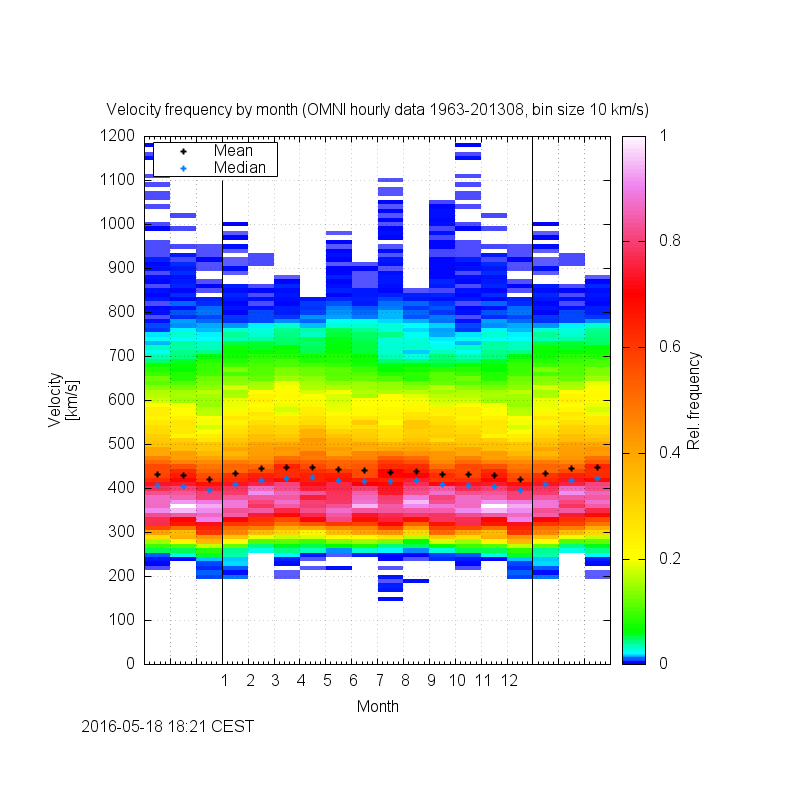
\includegraphics[width=0.3\textwidth]{images/gnuplots/OMNI_monthly_freq_V_gps.png}
	\caption{Diagram of the velocity frequency by month for the period 1963/01--2013/08. Mean and median values are shown as well.}
	\label{fig:OMNI_monthly_freq_V_gps}
\end{figure}

see \autoref{fig:OMNI_monthly_freq_B_a_gps}
\begin{figure}[htb]
	\centering
	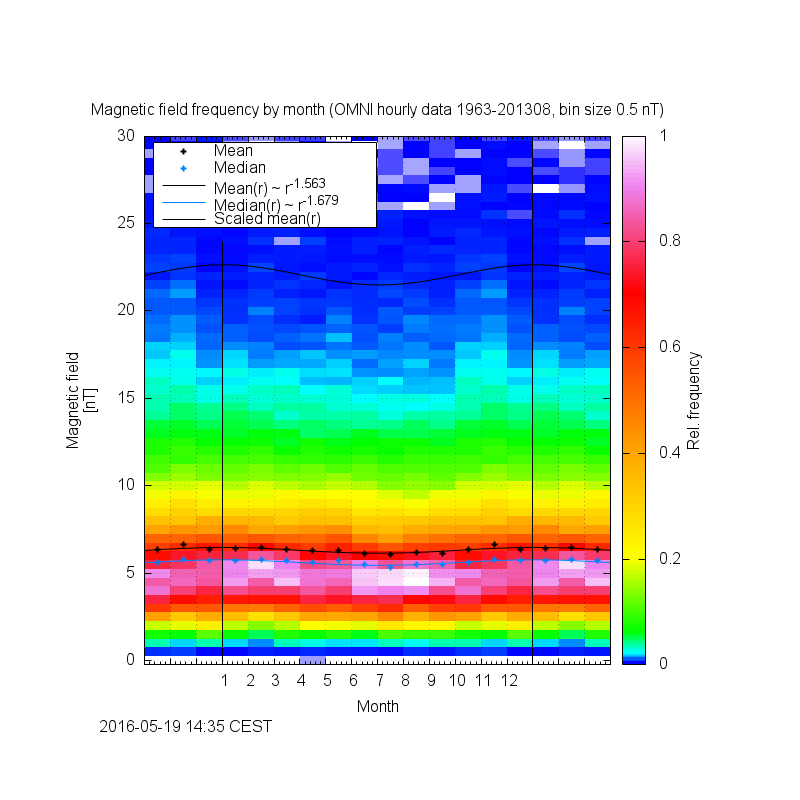
\includegraphics[width=0.3\textwidth]{images/gnuplots/OMNI_monthly_freq_B_a_gps.png}
	\caption{Diagram of magnetic field frequency by month for the period 1963/01--2013/08. Mean and median values are shown as well as the expected course from the solar distance variation (obtained from Helios data).}
	\label{fig:OMNI_monthly_freq_B_a_gps}
\end{figure}

derived exponent values from simple trigonometric fit on monthly values:\\
$c_N = -2.234$\\
maybe figure?\\

expected influence from Earth's perihelion/aphelion (see Appendix...) distance vs observations\\
we expect for the proton density (scaling law $N(r) = 7.6~\text{cm}^{-3} \cdot r^{-2}$):\\
N(0.983~au) = 7.9~cm$^{-3}$\\
N(1~au) = 7.6~cm$^{-3}$\\
N(1.017~au) = 7.3~cm$^{-3}$\\
we expect for the magnetic field strength (scaling law $\propto r^{-1.6}$):\\
B(0.983~au) = 6.3~nT\\
B(1~au) = 6.1~nT\\
B(1.017~au) = 5.9~nT\\


\section{Latitude dependency}
refer to Ulysses \autoref{fig:McComas2008_Ulysses_orbit}\\
Ulysses swoops polar plots...\\

see Schwenn1990's~Fig.~3.14\\
see also \citet{Schwenn1990} p.~127\\
see also \citet{Richardson1995}\\
Balogh et al. (1999) p. 162 ff (origin and formation of CIRs in inner heliosphere with Helios data; latitude V dependence)\\

latitude; see \autoref{fig:latitude_frequency_4_thesis_plot}
\begin{figure}[htb]
	\centering
	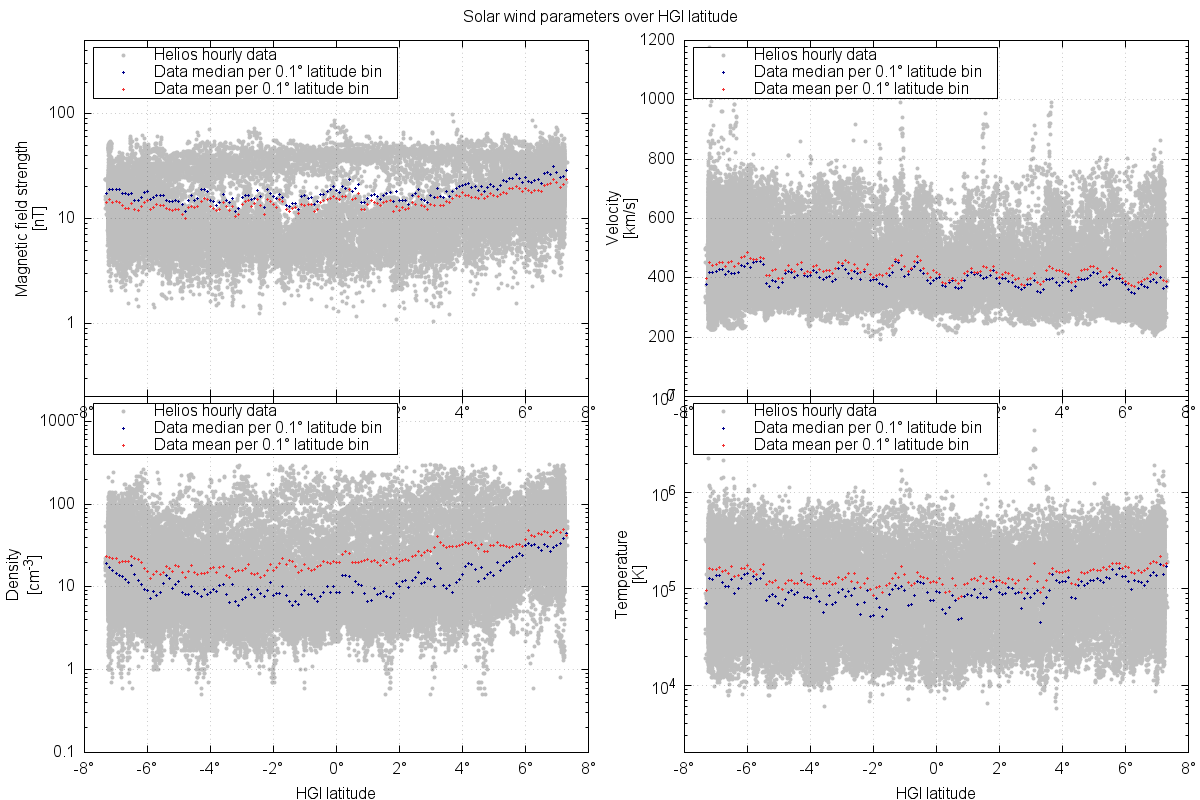
\includegraphics[width=0.5\textwidth]{images/gnuplots/latitude_frequency_4_thesis_plot.png}
	\caption{The four solar wind parameter's HGI latitude dependency. Their mean values per 0.1° bin are plotted as well. make figure same dimensions as projected figure in analysis part...}
	\label{fig:latitude_frequency_4_thesis_plot}
\end{figure}

with the exponential dependencies to 1~au projected solar wind parameters; there are only small changes with latitude in the range \SIrange{-7.25}{7.25}{\degree}\\
have a look on distribution widths...\\

dependence from latitude in interval -7.25°--7.25° in Helios data negligible?, see \autoref{fig:latitude_frequency_rcorrected_v3_4_thesis_plot}.
\begin{figure}[htb]
	\centering
	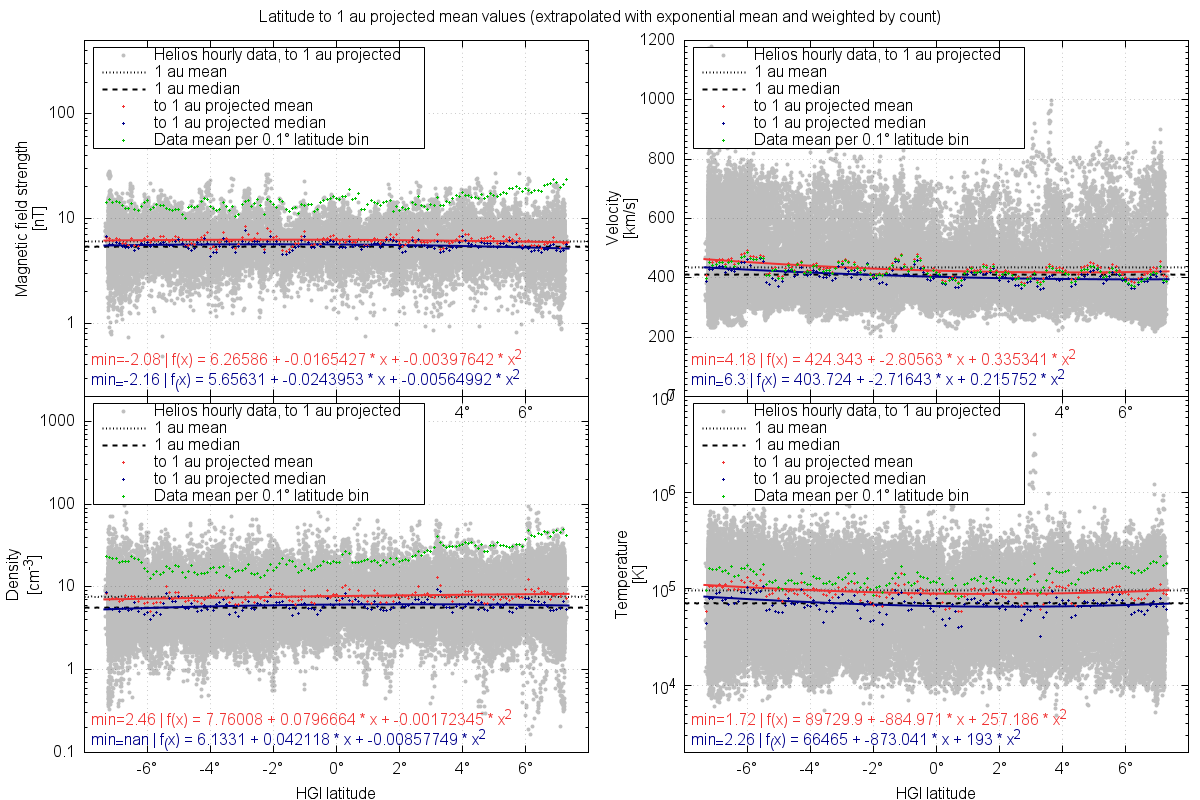
\includegraphics[width=0.5\textwidth]{images/gnuplots/latitude_frequency_rcorrected_v3_4_thesis_plot.png}
	\caption{Plot of the to 1~au projected solar wind parameters over latitude. And their mean values, including weighted fit. add projected median...}
	\label{fig:latitude_frequency_rcorrected_v3_4_thesis_plot}
\end{figure}
estimate error ranges...\\

...plot Ulysses data into plot?\\

%latitude variation negligible?
influence from latitude variation in data negligible? (see Ulysses \autoref{fig:McComas2008_Ulysses_orbit} in introduction). Helios probes within ecliptic => variation span equal to solar tilt: -7.25° to 7.25°; solar tilt/obliquity to ecliptic: $i_\odot = 7.25\degree$ (Sun fact sheet: \url{http://nssdc.gsfc.nasa.gov/planetary/factsheet/sunfact.html)}\\
big part of Helios data is from latitudes $>\pm5$°, see Figure~XX (data count over latitude) and see \autoref{fig:Helios12_orbits_ecliptic_polar} (Helios orbit polar plane in data section)\\


\section{Radial evolution of solar wind structures}
%see CGAUSS report2015_2

Helios event lists HSSs, SLOWs, CIRs, CMEs...; event lists for all Helios data\\
see Liu2004 for Helios ICME list and radial dependencies of $B$, $n$, $T$ and $v$...\\

\SI{200}{\km\per\s} slow solar wind at 10~$R_\odot$ is in agreement with blob measurements from Wang2000\\

very slow sw (VSSW) gets accelerated; see Sanchez-Diaz2016:\\
%"The reported in situ measurements suggest that the properties of VSSW are a continuation of the slow wind toward lower speeds: higher densities, higher proton fluxes, and lower temperatures, thereby extending well-known scaling laws [Lopez and Freeman, 1986; Hundhausen et al., 1970] down to speeds as low as 200 km/s."\\
%"The VSSW has a number of interesting properties that suggest it may be the interplanetary signature of long HPS crossings."\\


radial diameter of MCs increase between 0.3~au and 4.3~au proportional to the distance as $r^{0.8}$ \citep{Bothmer1998}\\
MC central axial magnetic field strength radial density dependence $B = 18.1\,r^{-1.64}$ \citet{Leitner2007}\\
MC average diameter $D = 0.23\,r^{1.14}$ \citet{Leitner2007}

sw structure marked plots\\

structure extrapolations\\


\section{sw parameters and precision}
definition of 'the four solar wind parameters':\\	%by OMNI histograms
	magnetic field strength, aka magnetic field, $B$, usually measured in nT, in the order of 0--35~nT at 1~au\\
	proton bulk velocity, aka velocity, $v$, usually measured in km/s, in the order of 200--900~km/s at 1~au\\
	proton number density, aka density, $n$, usually measured in cm$^{-3}$, in the order of 1--60 at 1~au\\
	proton temperature, aka temperature, $T$, usually measured in K, in the order of 10\,000--1\,000\,000~K at 1~au\\
sentence about ordering of the parameters...\\

%data binning
hourly OMNI data\\
measurement precision:\\
$B$: 0.01~nT\\
$v$: 1~km/s\\
$n$: 0.1~cm$^{-3}$\\
$T$: 1~K ? (smallest found: 7~K)\\

error discussion:\\
OMNI hourly data mean:\\
$B$: bin size 0.5~nT, median 5.6, mean 6.30056(18)\\
$v$: bin size 10~km/s, median 414, mean 437.6700(18)\\
$n$: bin size 1~cm$^{-3}$, median 5.3, mean 6.831410(18)\\
$T$: bin size 10\,000~K, median 80\,751, mean 112\,219.0(19) (with 1000~K as precision)\\

empirical data; Helios; hourly\\
why hourly and not higher resolution data?\\
measurement precision:\\
$B$: 0.01~nT\\
$v$: 0.1~km/s\\
$n$: 0.1~cm$^{-3}$\\
$T$: 100--1000~K (3 digits)\\
$r$: 0.01~au\\

error discussion:\\
Helios hourly data mean:\\
$B$: min 337, precision: 0.000545; 18.3x better\\
$v$: min 497, precision: 0.00449; 22.2x\\
$n$: min 497, precision:  0.00449; 22.2x\\
$T$: min 497, precision: 4.49--44.49 22.2x\\
=> so we use 1/10 the measurement precicion for the mean.\\

median precision same as data precision\\

%data binning
Helios histogram bin size for mean of frequency distribution (at specific solar distance)\\
$B$: bin size 0.5~nT, min 337, mean precision: 0.000545\\
$v$: bin size 1~cm$^{-3}$, min 497, mean precision: 0.00449\\
$n$: bin size 10~km/s, min 497, mean precision:  0.00449\\
$T$: bin size 10\,000~K, min 497, mean precision: 4.49--44.49\\


\section{other}
McGregor2011 analyzed the empirical magnetic topology–velocity relationship, using Helios perihelion data with the Wang-Sheeley-Arge (WSA) coronal model, and found indications, that the fast and slow solar wind are generated from distinct sources. (not only superradial expansion)\\

%GUM statement
Concerning the error notation I adhere to the parentheses notation documented in the ``Guide to the expression of uncertainty in measurement'' (GUM) published by \citet{GUM2008}, where the numbers in parentheses are the errors on the corresponding last digits of the quoted value.\\

For more on lognormal distributions see appendix \autoref{sec:lognormal_distribution}\\


%\captionsetup{width=0.75\textwidth}
%align caption width with table width  OR  widen table to textwidth?

%gnuplot:
%sum of the squared differences or 'residuals' (SSR) between the input data points and the function values, evaluated at the same places. This quantity is often called 'chisquare' 
%'stdfit', the standard deviation of the fit, which is the rms of the residuals, and the variance of the residuals, also called 'reduced chisquare' when the data points are weighted.
%The 'sum of squares of residuals', also called 'chisquare', is the WSSR between the data and your fitted function; fit has minimized that.
%The WSSR can be used to calculate the reduced chisquare (WSSR/ndf) or stdfit, the standard deviation of the fit, sqrt(WSSR/ndf). Both of these are reported for the final WSSR.


The extrapolation distance is only about one third of the model range, but as the parameters follow exponential change, one has to look at the logarithmic distance which is indeed one and a half times the model range.\\



